% !TEX root = deplump.tex
\section{Algorithm}
\newcommand{\T}{\ensuremath{\mathcal{T}}}
\newcommand{\N}{\ensuremath{\mathcal{N}}}
\newcommand{\M}{\ensuremath{\mathcal{M}}}
\newcommand{\PP}{\ensuremath{\mathcal{P}}}
\newcommand{\nc}{\ensuremath{nc}}
\newcommand{\RS}{\ensuremath{\mathcal{R}\mathcal{S}}}
\newcommand{\D}{\ensuremath{\mathcal{D}}}
\newcommand{\la}{\ensuremath{\leftarrow}}
\newcommand{\G}{\ensuremath{\mathcal{G}}}
\newcommand{\IS}{\ensuremath{\mathcal{I}\mathcal{S}}}
\newcommand{\Seq}{\ensuremath{\mathcal{S}}}
\newcommand{\dd}{\ensuremath{\delta}}
%
%\begin{figure*}[t] 
%	\begin{center}
%		\scalebox{.6}{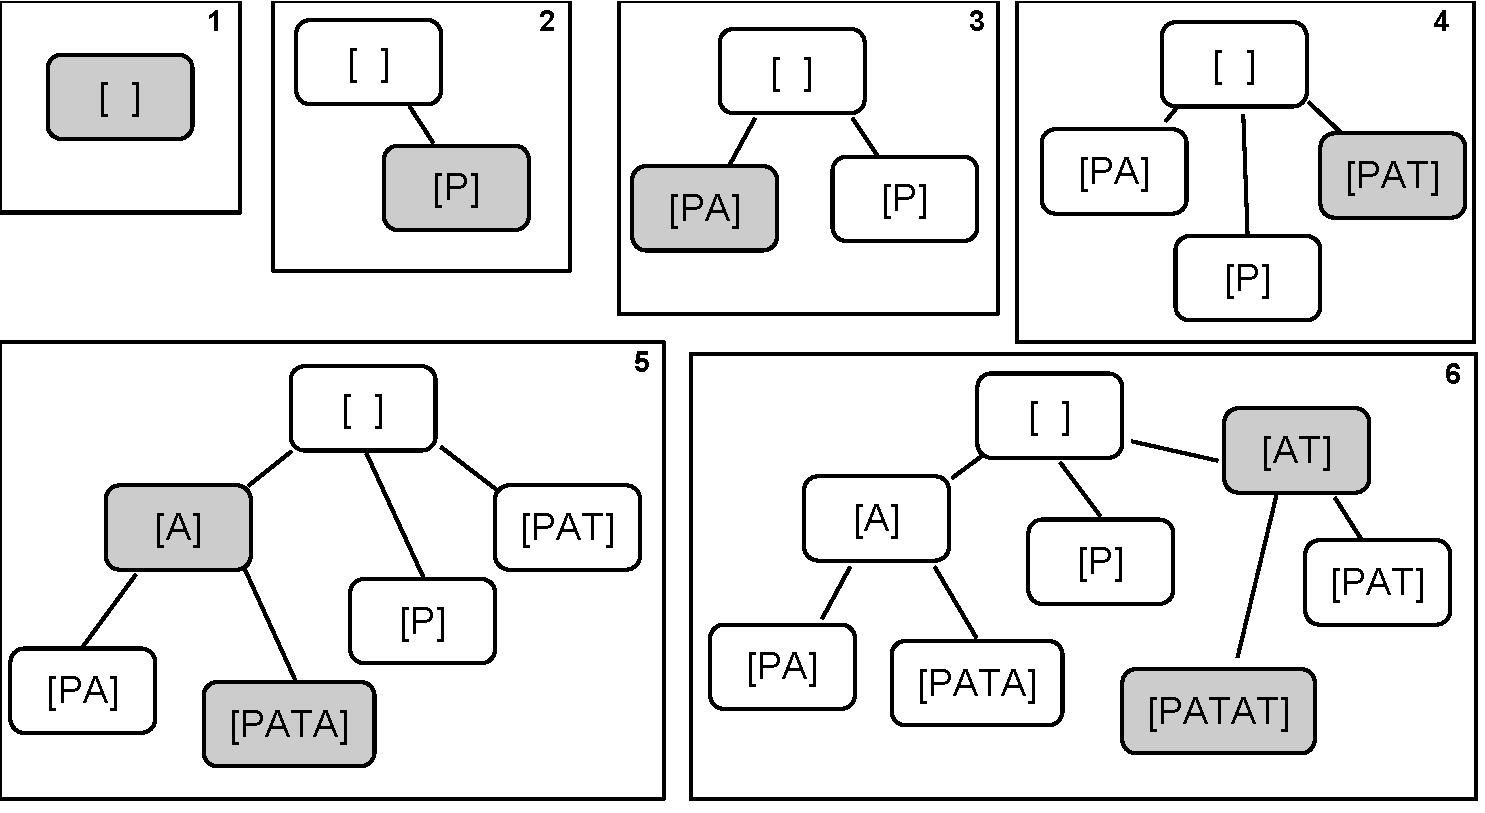
\includegraphics{figs/PATAT.pdf}} % [clip=true, viewport= 1in 1in 9in 9in]
%		\caption{Construction of suffix tree for string ``PATAT".  In each frame the new nodes are shaded in gray.}
%		\label{fig:suffix_tree}
%	\end{center} 
%\end{figure*} 
%
Given a sequence of symbols $\Seq = [s_0, s_1, s_2, \ldots]$ where each symbol $s_n$ comes from from an ordered set of symbols $\{\sigma_0, \sigma_1, \ldots\} = \Sigma$,  deplump works by repeatedly producing a predictive distribution for the continuation of the sequence given the full preceding context and encoding the next symbol by passing that predictive distribution to an entropy encoder.  In this paper explicit details related to encoding and decoding are not included, instead we present the algorithms necessary to incrementally construct the predictive distributions needed by the encoder and decoder.  Specifically, we assume that if the predictive distribution function is $F$ and the next symbol in the stream is $s$ then the stream can be compressed using an entropy encoder that takes $F(s-1)$ and $F(s)$ as arguments and returns a bit stream (possibly null)\citep{Witten1987,arithmeticencoding}.   The cumulative distribution function is well defined because the symbols are ordered. We use the notation $s-1$ to refer to the symbol prior to $s$ in the symbol set $\Sigma$.  %Note that the symbol set can be ordered as the set is discovered.

The algorithms of deplump run over an incrementally constructed suffix-tree-like data structure \citep{Ukkonen1992}. This data structure efficiently encodes the set of unique suffices of all contexts in a sequence (i.e.~the set $\{ [ ], [s_0], [s_0,s_1], [s_0, s_1,s_2], \ldots \}$).  Each node in the tree corresponds to a subsequence $[s_m, \ldots, s_{m + k}]$ of the input sequence.  We use $\N$ to refer interchangeably to a node and the subsequence to which the node corresponds.  Each edge in the tree is labeled by a subsequence of the input sequence.  On each edge we use indices $i$ and $j$ to indicate that the edge label is $[s_{i+1}, s_{i+2}, \ldots,s_{j}]$. For a given suffix the location of the corresponding node can be found by traversing edges of the tree that match the suffix read from right to left. 

\begin{algorithm}[t]
    \caption{Deplump/Plump} \label{alg:deplump/plump}
    \begin{algorithmic}[1]
    	\Procedure{Deplump/Plump}{$\IS$}
		\State $\RS \la [$ $]  $ \Comment{reference sequence}
		\State Initialize $[$ $]$ node of \T \Comment{suffix tree}
		\State $\nc \la 1$ \Comment{node count}
		\State $\D \la  \{ \dd_0, \dd_1, \dd_2, \dots, \dd_{10}, \alpha \}$ \Comment{discount parameters}
		\State $\G \la \vec 0$ \Comment{discount parameter gradients, $|\G| = |\D|$}
		\State $\mathcal{O}\mathcal{S} \la  [$ $]$ \Comment{output sequence}
		\For{i = 1: $| \IS|$}
			\State [$\pi$, \N] $\la$ \textsc{PMFNextSymbol} (\RS)
			\If{Plump}
				\State $s \la $ \textsc{RangeDecode}($\pi$, \IS)
				\State $\mathcal{O}\mathcal{S} \la [\mathcal{O}\mathcal{S}$ $s]$
			\Else
				\State $s \la \IS[i]$
				\State $b \la$ \textsc{RangeEncode}$(\Sigma_{i = 1}^{s-1} \pi_i, \Sigma_{i = 1}^{s} \pi_i$)
				\State $\mathcal{O}\mathcal{S} \la [\mathcal{O}\mathcal{S}$ $b]$		
			\EndIf
			\State \textsc{UpdateCountsAndDiscountGradients}($\N,s,\pi_s,$TRUE)
			\State $\D \la \D + \G \eta / (\pi_s)$ \Comment{update discount parameters}
			\State $\G \la \vec 0$ \Comment{reset gradients to zero}
			\State $\RS \la [\RS$ $s]$ \Comment{append symbol to reference sequence}
		\EndFor
		\State \Return $\mathcal{O}\mathcal{S}$
	\EndProcedure
	\end{algorithmic}
\end{algorithm}

Algorithm~\ref{alg:deplump/plump} shows that deplump processes each element of an input sequence $\IS$ in succession.  For each element $s_n$ of $\IS$, \textsc{PMFNextSymbol} is called to retrieve the predictive probability mass function $\pi$ (conditioned on the observed context $[s_0, s_1, \ldots, s_{n-1}] = \RS$).  The element $s_n$ is then encoded by an entropy encoder with parameter $\pi$.  The counts in the tree are updated and the gradients for the discount parameters are calculated by \textsc{UpdateCountsAndDiscountGradients}. The discount parameters are updated based on a learning rate $\eta$ and the encoded symbol in appended to $\RS$.

The first two steps of \textsc{PMFNextSymbol} concern upper bounds on $|\RS|$ and $|\mathcal{H}|$.  First, since the labeling of edges in the tree reference $\RS$, when it is shortened, some edges may become unlabeled.  Those edges are removed from the tree along with all the nodes in the subtrees below them. To minimize the number of nodes removed this way, the edge indices are updated as the algorithm progresses to reference recent sections of $\RS$. Second, if the number of nodes in the tree approaches the limit $L$ then random leaf nodes are removed.  A leaf node is a node with no descendants. To facilitate their random deletion we maintain a count in each node of the number of leaf nodes in the subtree below it.  A random leaf node can be obtained by traversing a weighted random path down the tree.  The third step of \textsc{PMFNextSymbol} retrieves the appropriate node for prediction by calling \textsc{GetNode}. The predictive probability mass function is calculated by \textsc{PMF}.

Since the model is estimated incrementally, the tree data structure must also be incrementally constructed.  Construction of the tree is handled by the function \textsc{GetNode} within \textsc{PMFNextSymbol}.  Within the function \textsc{GetNode}, nodes are created by \textsc{CreateNode} and \textsc{FragmentNode}. The function \textsc{CreateNode(\N,\M)} creates a node $\N$ with parent $\M$. \textsc{FragmentNode} implements the fragmentation operation developed in \citep{Wood2009} and is called when none of the existing tree nodes are a suffix of the context.  %An illustration of the incremental construction of a suffix tree can be seen in Figure~\ref{fig:suffix_tree} for the toy sequence [PATAT].  We use \textsc{PA}(\N) to refer to the parent of $\N$ in the tree.  In frame 4 the function \textsc{GetNode} assigns [ ]  to $\M$ and then [PAT] to $\Seq$ with $\M = \textsc{PA}(\Seq)$. In Frame 5 \textsc{GetNode} assigns [PA] to $\M$, but then must assign [A] = \textsc{FragmentNode}(\M) to $\PP$ and \textsc{PA}$(\M)$ to \PP.  Node $\Seq$ is then created by \textsc{CreateNode}$($[PATA]$,\PP)$.   % In each frame the first step is to find $\M$, which can be achieved by descending an appropriate path of the suffix tree.  All of the nodes on the path to $\M$ and possibly $\M$ itself can have the indices into $\RS$ updated to point to a more recent section of the reference sequence. 

Each node instance $\N$ contains two counts for each $\sigma \in \Sigma$, $c_\sigma$ and $t_\sigma$.  We use $c$ and $t$ to refer to the marginal counts $\sum_{\sigma \in \Sigma} c_\sigma$ and $\sum_{\sigma \in \Sigma} t_\sigma$.  Each node also has a discount associated with it which we refer to as $d^\N$ in the algorithms. If we define $\delta_{n} = \delta_{10}^{\alpha^{n - 10}}$ for $n \geq 10$ then $d^{\N} = \Pi_{i =|\textsc{PA}(\N)| + 1}^{|\N|} \delta_{i}$ if $\N$ is not the root and $\delta_{0}$ if $\N$ is the root.  Counts are updated and discount parameter gradients are calculated by Algorithm~\ref{alg:updatecountsandgradients}.  The new approximation discussed in Section~\ref{section:methodology} is implemented by \textsc{ThinCounts}.

%The reference sequence grows with the length of the input sequence and must be shortened as the algorithm progresses.  When $\RS$ is shortened, nodes in the suffix tree which reference removed sections are no longer usable and must be removed from the tree to prevent a memory leak.  To facilitate the removal process pointers are maintained from the elements of $\RS$ to the suffix tree nodes which reference them.  Without the use of pointers, deletion of the unusable nodes requires a search over the tree which is prohibitive for large trees. The cost of these operations can be amortized by shorting $\RS$ in chunks and keeping pointers from each chunk of $\RS$ instead of each element.  

%The reference sequence $\RS$ is implemented as a linked list. Therefore, instead of using a simple $i,j$ index in each suffix tree node, $i$ is replaced by a linked list node and an offset and $j$ is replaced by a string length $l$.  Each node of the linked list must contain a list of suffix tree nodes which reference it.  The reference sequence grows as the length of the input sequence grows and must be shortened as the algorithm progresses.  The shortening of $\RS$ is made explicit by the $\sigma$ operator in CDFNextSymbol, which returns the argument sequence shortened by removing the fist element.  When $\RS$ is shortened, nodes in the suffix tree which reference removed sections are no longer usable and must be removed from the tree to prevent a memory leak.  Without a list of suffix tree nodes which reference each linked list node, deletion of the unusable nodes requires a search over the tree which is prohibitive for large trees.  The cost of these operations can be amortized by shorting $\RS$ in chunks, i.e. by removing nodes of the linked list.  To minimize the impact of rendering nodes unusable by shortening the reference sequence, nodes should be updated to point to the most recent part of $\RS$ as possible.

The function \textsc{Multinomial} is used in several of the algorithms and returns a single value sampled from a discrete distribution.  The two parameter Ewen's $(\mathcal{E}\mathcal{S}_{n}(d,c))$ distribution is a distribution over partitions of $n$ objects and often plays a key role in inference for models using Pitman-Yor distributions \cite{Ewens_dist_ref}.  The  distribution shows up here in the functions \textsc{DrawCRP(n,d,c)}, which is called in \textsc{FragmentNode}, \textsc{Partition}.   \textsc{DrawCRP(n,d,c)} returns the length of a random partition drawn from the $\mathcal{E}\mathcal{S}_{n}(d,c)$.  The function \textsc{Partition(c,t,d)} implements the seating arrangement reconstruction algorithm discussed in \citep{Gasthaus2011} to sample a partition following the $\mathcal{E}\mathcal{S}_{c}(d,0)$ distribution conditioned that the length of the partition be $t$.

Several parameters required by the model must be assigned at initialization.  They are $\D$, $D$, $T$, $k$, $L$, $\eta$,  and depth.  $\D = [\dd_0, \dd_1, \ldots, \dd_{10}, \alpha]$ is a list of discount parameters, each taking a real value in $(0,1)$.  $D$ is maximum length of suffices considered when creating the suffix tree.  $T$ is an upper bound on the length of $\RS$.  The parameter $k$ is positive integer valued and is an upper bound on the total count $c$ in each node.  The parameter $L$ is an upper bound on the number of node instances in the suffix tree. The parameter $\eta$ is a learning rate for the updating of the discount parameters and is typically set very small.  

%For each $s$ in the input sequence the function \textsc{PMFNextSymbo}l is called to obtain the predictive probability mass function (PMF).  After encoding or decoding using the predictive PMF $pi$ the first step in updating the model estimate is performed by the function \textsc{UpdateCountsAndDiscounts}.  Starting at node $\N$ and progressing up to the root of the tree, $c_s$ is incremented if $t_s$ was incremented in the node below.  If $c_s$ is incremented, a stochastic decision is made to increment $t_s$.  The gradients for the discount parameters $\D$ are updated by the function \textsc{UpdateDiscountParameterGradients}.  If $c$ is larger than $k$ in any of the nodes, the counts $c_s$ and potentially $t_s$ are reduced by the function \textsc{ThinCounts}. Finally, \D \space is updated based on the calculated gradients and the specified learning rate $\eta$ and the symbol is appended to \RS.

\begin{figure*}[ttt!]
	\begin{minipage}[t]{.48\linewidth}
		\begin{algorithm}[H]
			\caption{PMFNextSymbol} \label{alg:pmfnextsymbol}
	\begin{algorithmic}[1]
	\Function{PMFNextSymbol}{$\RS$}
		\While{$ |\RS| \geq T$}
%			\State Delete nodes referencing \RS[1] and update $nc$
			\State $\RS \la \sigma(\RS)$
		\EndWhile
		\While{ $\nc > (L - 2)$}
			\State Delete random leaf node
			\State $nc \la nc -1$
		\EndWhile
		
		\State $\N \la$ \textsc{GetNode}$(\RS, \T)$
		\State $\pi \la$ \textsc{PMF}($\N, \vec 0, 1.0$) \Comment{$| \vec 0| = | \Sigma|$}
	%	\State UpdateCountsAndDiscountGradients($\N,s,\pi_s,$TRUE)
		\State \Return [$\pi$, \N]
	\EndFunction
	 \end{algorithmic}
\end{algorithm}
	 \end{minipage}
	\hfill
%
%
%%\begin{algorithm}
%	\caption{GetDiscount} \label{alg:getdiscount}
%    \begin{algorithmic}[1]
%    	\Function{PointOnCDFNextSymbol}{$h,\T,\RS$}
%		\While{$ |\RS| \geq 100 L$}
%			\State Delete nodes referencing \RS[0]
%			\State $\RS \la \sigma(\RS)$
%		\EndWhile
%		\While{ $\nc > (L - 2)$}
%			\State Delete leaf node uniformly at random
%		\EndWhile
%		\State $\N \la$ GetNode$(\RS, \T)$
%		\State $\pi \la$ PMF($\N, \vec 0, 1.0$) \Comment{$| \vec 0| = | \Sigma|$}
%		
%		\State $F(s) \la 0$
%		\State $s \la 0$
%		\While{$F(s) < h$}
%			\State $s \la s + 1$
%			\State $F(s) \la F(s) + \pi_s$
%		\EndWhile
%		
%		\State $F(s-1) \la F(s) - \pi_s$
%		\State Update $h$
%		\Return  $[h,s, F(s-1), F(s)]$
%	\EndFunction	
%	\Function{GetDiscount}{\N}
%		\State $d = 1.0$
%		\If{\N = [ ]}
%			\State \Return $\dd_0$
%		\EndIf
%		\For{$i = (|$\textsc{PA}$(\N)| + 1): |\N|$}
%			\If{$i \leq 10$}
%				\State $d \la d \delta_i$ \Comment{multiply by discount parameter $i$}
%			\Else
%				\State $d \la d \dd_{10}^{\alpha^i}$
%			\EndIf
%		\EndFor
%		\State \Return $d$
%	\EndFunction
%	
%		\end{algorithmic}
%\end{algorithm}
	\begin{minipage}[t]{.48\linewidth}
\begin{algorithm}[H]
	\caption{GetNode} \label{alg:getnode}
	\begin{algorithmic}[1]
    	\Function{GetNode}{\Seq, \T}
		\State Find the node \M \space in the tree sharing the longest suffix with \Seq
		\If{\M \space is a suffix of \Seq}
			\If{$\Seq = \M$ or $|\M| = D$}
				\State \Return \M
			\Else
				\State $\Seq \la$ \textsc{CreateNode}$(\Seq, \M)$
				\State $nc \la nc + 1$
				\State \Return \Seq
			\EndIf
		\Else
			\State \PP \la \space \textsc{FragmentNode}(\M, \Seq)
			\State $\Seq \la $ \textsc{CreateNode}$(\Seq, \PP)$
			\State $nc \la nc + 1$
			\State \Return \Seq
		\EndIf
	\EndFunction
	\end{algorithmic}	
\end{algorithm}
	\end{minipage}
	\end{figure*}
	

\begin{algorithm}
	\caption{UpdateCountsAndDiscountGradients} \label{alg:updatecountsandgradients}
	\begin{algorithmic}[1]
	
	\Function{UpdateCountsAndDiscounts}{$\N, s, p$, BackOff}
	%	\State $d \la $ \textsc{GetDiscount}(\N)
		\State $pp \la p$
		\If{$c > 0$}
			\State $pp \la (p - \frac{c_s - t_s d^{\N}}{c}))(\frac{c}{t d^{\N}})$
			\State $w \la c_s	+ d^{\N}(t *pp - t_s)$		
		\EndIf
		
		\If{BackOff  and $c > 0$}
			\State $c_s \la c_s + 1$
			\State BackOff $\la 0$
			\State BackOff $\la 1$ w.p. $pp (\frac{t d^{\N}}{w})$ \Comment{w.p abbreviates ``with probability"}
			\If{BackOff}
				\State $t_s \la t_s + 1$
			 \EndIf
		\ElsIf{BackOff}
				\State $c_s \la c_s + 1$;  $t_s \la t_s + 1$
		\EndIf
		\State \textsc{UpdateDiscountParameterGradients}($t_s, t,pp, d^{\N}$)
		\State \textsc{UpdateCountsAndDiscountGradients}(\textsc{PA}(\N), $s,pp$, BackOff)
		\State \textsc{ThinCounts}(\N)
	\EndFunction
		\end{algorithmic}
\end{algorithm}

\begin{figure*}[ttt!]
\begin{minipage}[t]{.48\linewidth}
\begin{algorithm}[H]
	\caption{ThinCounts} \label{alg:thincounts}
	\begin{algorithmic}[1]
			
	\Function{ThinCounts}{$\N$}
	%	\State $d \la$ \textsc{GetDiscount}$(\N)$
		\While{$c > k$}
			\State $\pi_{l} = \frac{c_l}{c}$, $l = 1, \ldots, |\Sigma|$
			\State $s \la $ \textsc{Multinomial}$(\pi)$ %s.t. $\pi_l = \frac{c_l}{c}$ % \Comment{$\pi$ is a distribution over $\Sigma$}
			\State $\phi \la$ \textsc{Partition}$(c_s, t_s, d^{\N})$
			\State $\psi \la \frac{\phi}{c_{s}}$
			\State $i \la$ \textsc{Multinomial}$(\psi)$
			\If{$\phi_i == 1$}
				\State $t_s \la t_s - 1$
			\EndIf
			\State $c_s \la c_s - 1$
		\EndWhile
	\EndFunction	
	
	\end{algorithmic}	
\end{algorithm}
\end{minipage}
\hfill
\begin{minipage}[t]{.48\linewidth}
\begin{algorithm}[H]
	\caption{PMF} \label{alg:pmf}
	\begin{algorithmic}[1]

	\Function{PMF}{$\N, \pi, m$}
%		\State $d \la $ \textsc{GetDiscount}(\N)		
		\If{$c > 0$}
			\For{$s \in \Sigma$}
				\State $\pi_s\la \pi_s + m(\frac{c_s - t_s d^{\N}}{c})$
			\EndFor
		\EndIf
		
		\If{\textsc{PA}$(\N) \neq$ null}
			\State \Return \textsc{PMF}(\textsc{PA}(\N), $\pi, d^{\N} m$)
		\Else
			\State $\pi \la (1- d^{\N} m)\pi + d^{\N}m\mathcal{U}_{\Sigma}$ %\Comment{$\mathcal{U}(\Sigma)$ is the uniform distribution over $\Sigma$}
			\State \Return $\pi$
		\EndIf 
	\EndFunction
		\end{algorithmic}
\end{algorithm}
\end{minipage}
\end{figure*}

\begin{algorithm}
	\caption{FragmentNode} \label{alg:fragmentnode}
	\begin{algorithmic}[1]

	
	\Function{FragmentNode}{$\M, \Seq$}
%		\State $d^\M \la$ \textsc{GetDiscount}(\M)
		\State $\PP \la$ maximum overlapping suffix  of \M \space and \Seq
		\State $\PP \la $ \textsc{CreateNode}$(\PP,$ \textsc{PA}$(\M))$
		\State $nc \la nc + 1$
		\State\textsc{ PA}(\M) $\la \PP$
%		\State $d^\PP \la$ \textsc{GetDiscount}(\PP)
		\For{$s \in \Sigma$}
			\State $\phi \la$ \textsc{Partition} $(c^\M_s, t^\M_s,d^\M)$
			\State $t^\PP_s \la t^\M_s$;  $t^\M_s \la 0$
			\For{$i= 1 : | \phi|$}
				\State $a \la$ \textsc{DrawCRP}$(\phi[i],d^\M / d^\PP,-d^\M)$
				\State $t_s^\M \la t_s^\M + a$
			\EndFor
			\State $c^\PP_s \la t^\M_s$
		\EndFor
		\State \Return \PP
	\EndFunction
		\end{algorithmic}
\end{algorithm}

%\begin{algorithm}
%	\caption{DrawCRP} \label{alg:drawcrp}
%	\begin{algorithmic}[1]
%
%	
%	\Function{DrawCRP}{$n,d,c$} \Comment{$ n \geq 1$}
%		\State $t \la 1$
%		\For{i = 2 : n}
%			\State $r \la 0$
%			\State $r  \la 1$ w.p. $\frac{td + c}{i-1 + c}$
%			\State $t \la t + r$
%		\EndFor
%		\State \Return $t$
%	\EndFunction
%	
%	\end{algorithmic}	
%\end{algorithm}

\begin{algorithm}
	\caption{Partition} \label{alg:samplepartition}
	\begin{algorithmic}[1]
	
	\Function{Partition}{$c,t,d$}
		\State $M \la  t \times c$ matrix of zeros
		\State $M(t,c) \la 1.0$
		\For{$j = (c-1) : 1$}
			\For{$i = 1 : (t-1)$} 
				\State $M(i,j) \la M(i +1, j+1) + M(i,j+1)(j - id)$ 
			\EndFor
			\State $M(d,j) \la M(t,j+1)$
		\EndFor
		\State $\phi \la \vec 0$ \Comment{$|\vec 0| = t$}
		\State $\phi[1] \la 1$;  $k \la 1$
		\For{j = 2 : c}
			\State $M(k,j) \la M(k,j)(j-1 -k d)$
			\State $r \la 0$
			\State $r \la 1 $ w.p. $\frac{M(k+1,j)}{M(k+1,j) + M(k,j)}$
			\If{r = 1}
				\State $k \la k + 1$
				\State $\phi[k]  \la 1$
			\Else
				\State $i \la$ \textsc{Multinomial}$([\frac{\phi[1] - d}{j-1 -kd}, \frac{\phi[2] - d}{j-1 -kd}, \ldots, \frac{\phi[k] - d}{j-1 -kd}])$
				\State $\phi[i] \la \phi[i] + 1$
			\EndIf
		\EndFor
		\State \Return $\phi$
	\EndFunction
		\end{algorithmic}
\end{algorithm}

%\begin{algorithm}
%	\caption{UpdateDiscountParameterGradients} \label{alg:updatediscountparametergradients}
%	\begin{algorithmic}[1]
%
%
%	\Function{UpdateDiscountParameterGradients}{$\N, t_s, c, t, pp, d, m$}
%		\If{$c > 0$}
%			\If{$|\N| = 0$}
%				\State $ \psi \la \frac{1.0}{\dd_0}$
%				\State $\G_0 \la \G_0 + (d(t * pp - t_s)\psi / c)  m$
%			\Else
%				\State $z \la |$\textsc{PA}(\N)$| + 1$
%				\While{$z \leq |\N|$ and $z < 10$}
%					\State $\psi \la \frac{1.0}{\dd_z}$
%					\State $\G_z \la \G_z + (d(t * pp - t_s) \psi / c)  m$	
%				\EndWhile
%				
%				\If{$|\N| \geq 10$}
%					\State $a \la z - 10$
%					\State $b \la |\N| - z + 1$
%					\State $\psi \la \alpha^a(1 - \alpha^b) / ((1 - \alpha)  \dd_{10})$ 
%					\State $\G_{10} \la \G_{10} + (d(t * pp - t_s) \psi / c)  m$	
%					\State $\psi \la$ log$(\dd_{10}) (a \alpha^{a-1} - (a + b)\alpha^{a + b-1}) / (1 - \alpha) + (\alpha^a - \alpha^{a + b}) / (1 - \alpha)^2$
%					\State $\G_{11} \la \G_{11} + (d(t * pp - t_s)\psi / c)  m$	
%				\EndIf
%			\EndIf
%		\EndIf
%	\EndFunction
%
%	\end{algorithmic}	
%\end{algorithm}
